% !TeX spellcheck = cs_CZ

% xelatex -enable-write18 -shell-escape mai_fig029.tex
\documentclass{standalone}
\usepackage{amsmath}
\usepackage{tikz}
\usetikzlibrary{decorations.markings}
\usetikzlibrary{intersections}
\usetikzlibrary{calc}

\begin{document}

  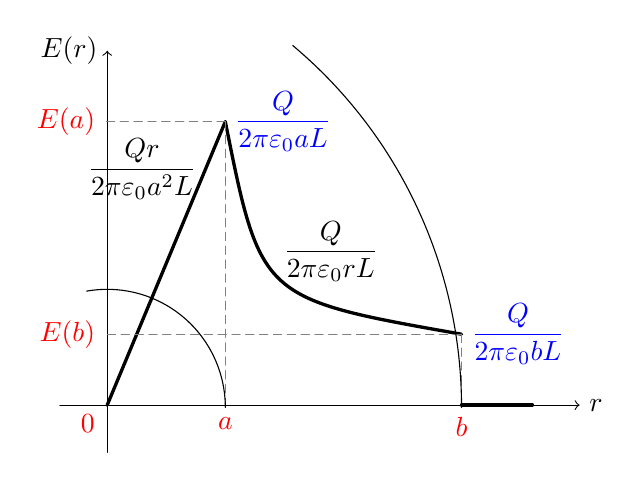
\begin{tikzpicture}
     [scale=3,line cap=round,
      % Styles
        axes/.style=,
        important line/.style={very thick},
        information text/.style={rounded corners,fill=red!10,inner sep=1ex}]
    \begin{scope}[axes]     
      \draw[->] (-0.2, 0) -- (2, 0)   node[right] {\(r\)} coordinate(x axis);
      \draw[->] (0, -0.2) -- (0, 1.5) node[left] {\(E(r)\)} coordinate(y axis);
      \draw[red](0,-0.08) node[left=1pt]{$0$};
    \end{scope}
    % my function  
    \coordinate [label={[blue] right:\(\dfrac{Q}{2\pi\varepsilon_0aL}\)}] (D) at (0.5,1.2);
    \draw[very thick] (0,0) -- (D);  
    \coordinate [label={[blue] right:\(\dfrac{Q}{2\pi\varepsilon_0bL}\)}] (C) at (1.5,0.3);
    \draw[very thick, name path=func] (D) .. controls (0.65,0.45) .. (C);
    \draw[very thick] (1.5,0) -- ++(0.3,0); % E = 0 line
    % horizontal line
    \draw[gray, densely dashed] (D) -- ++(0,-1.21) node[below, red]{$a$} coordinate(a);
    \draw[gray, densely dashed] (C) -- ++(0,-0.31) node[below, red]{$b$} coordinate(b);

    \draw[gray, densely dashed] (D) -- ++(-0.51,0) node[left, red]{\(E(a)\)} coordinate(Ea);
    \draw[gray, densely dashed] (C) -- ++(-1.51,0) node[left, red]{\(E(b)\)} coordinate(Eb);

    \draw (1.2,0.65) node[left=1pt]{\(\dfrac{Q}{2\pi\varepsilon_0rL}\)};
    \draw (0.43,1) node[left=1pt]{\(\dfrac{Qr}{2\pi\varepsilon_0a^2L}\)};

    % https://tex.stackexchange.com/questions/175016/how-is-arc-defined-in-tikz
    % \draw (x,y) arc (start:stop:radius);
    % with radius r
    % starts from (x,y)
    % with center (x-r*cos(start), y-r*sin(start)) and
    % ends at (x-r*cos(start)+r*cos(stop), y-r*sin(start)+r*sin(stop)).
    \draw (a) arc (0:100:0.5);
    \draw (b) arc (0:50:2);
  \end{tikzpicture}

\end{document}